% ==============================================
\section{Introduction}
\label{sec:intro}
% ==============================================
% Problem
Programmers often search for online code examples to learn new APIs. A case study at Google shows that developers issue an average of 12 code search queries per weekday~\cite{sadowski2015developers}. Stack Overflow (SO) is a popular Q\&A website that programmers often consult. In July 2017, Stack Overflow has accumulated more than 22 million answers, many of which contain code examples to demonstrate the solution for a particular programming question. However, SO examples are not always complete or reliable, which can be misleading and potentially dangerous when programmers follow the same example to complete a client program. For example, Fischer et al.~found that 29\% of security-related code snippets on Stack Overflow were insecure and have potentially affected over 1 million Android apps on Google play~\cite{fischer2017stack}. 

% Solution
This paper presents {\tool}, a Chrome extension that augments Stack Overflow with common API usage patterns learned from GitHub and alerts programmers about the potential violations in a Stack Overflow post. Current {\tool} includes hundreds of API usage patterns learned from 380K GitHub repositories.\footnote{The entire dataset of patterns is uploaded with EasyChair.} These patterns represent three types of API-related usage---temporal ordering, guard conditions, and exception handling logic of API methods. Our insight is that commonly practiced idioms in massive code corpora may represent a desirable pattern that a programmer can use to trust and enhance code examples on Stack Overflow. 

Given a Stack Overflow post, {\tool} first extracts the sequence of API calls with corresponding control constructs and guard conditions. {\tool} then contrasts the sequence with the dataset of API usage patterns learned from GitHub and highlights method calls that violate the common usage patterns. To help users better understand the violations, {\tool} further generates descriptive warning messages and also suggests a corrected usage example with the same variable names as in the Stack Overflow code snippet. Mining API usage patterns to detect violations often suffers from reporting false alarms, since mined patterns may not be inclusive and fit all use scenarios of an API~\cite{liang2016antminer}. To mitigate this issue, {\tool} allows users to upvote or downvote a violation based on its applicability and usefulness to a Stack Overflow post. {\tool} filters a pattern when multiple users flag it unhelpful to constrast against a given snippet. To help developers build confidence on a detected violation, {\tool} shows how many GitHub developers also follow the pattern as well as how many other users like or dislike this pattern.

\begin{figure}
\centering
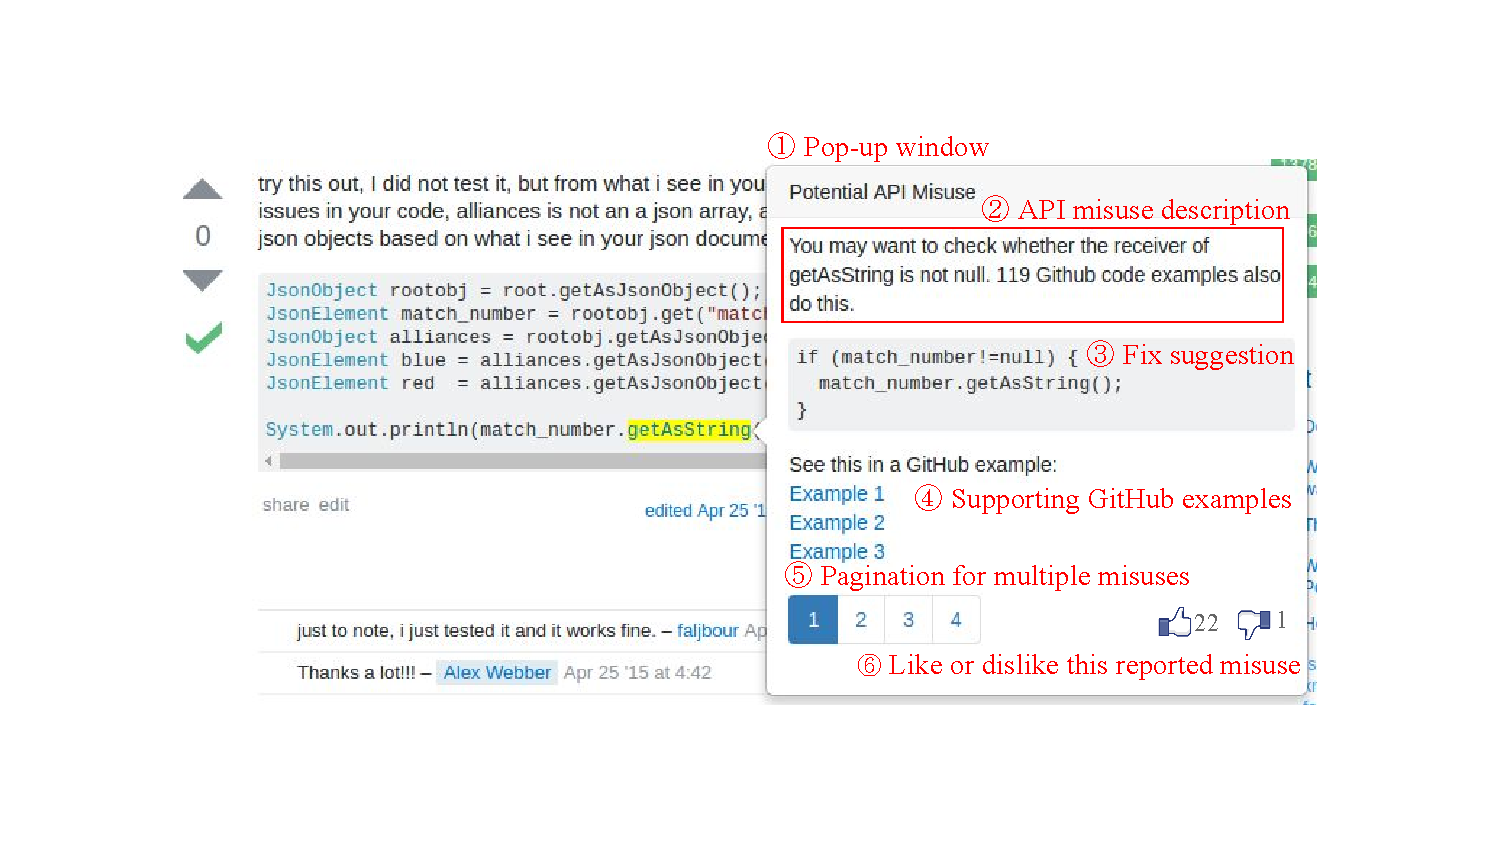
\includegraphics[width=0.5\textwidth]{soap-v3.pdf}
  \vspace{.1in}
  \caption{{\tool} Chrome extension that augments Stack Overflow with API misuse warning. The pop-up window alerts that {\ttt match\_number} can be {\ttt null} if the requested {\ttt JSON} attribute does not exist and will crash the program by throwing {\ttt NullPointerException} when {\ttt getAsString} is called on it.\protect\footnotemark}
  \label{fig:screenshot}
\end{figure}

\footnotetext{\url{https://stackoverflow.com/questions/29860000}}

A user of {\tool} would benefit from the addition of concrete examples from the production code in GitHub  to the code examples she encounters on Stack Overflow. This will not only combat programming issues stemming from the use of incomplete or unreliable Stack Overflow code examples, but will also be an aid for users learning a new API. By enhancing examples already found in Stack Overflow, a user can trust that the shown example follows a common and reliable usage pattern for a given API method.
%A user of this tool would benefit from not needing to cross-reference multiple sites for proper API usage reference, and will be able to continue using Stack Overflow to learn APIs with the added advantage of seeing which usage patterns a post may have left out of its explanation. This could result in more complete, reliable code with minimal added time or effort on the part of the programmer.\todo{The description here does not sound very appealing. Can you rework this paragraph?} 

The main contribution of this paper is to describe the features of {\tool} from a user's perspective. In order to give programmers access to {\tool}, the front-end of {\tool} is implemented as a Chrome extension that users can easily download and install.\todo{add a url to download our tool} The detailed algorithm and study are described in our separate technical report.\todo{cite Maple}

%input{fig_motiExample}
%\input{fig_UI}
